% arara: pdflatex

\documentclass[12pt,a4paper, landscape]{article}
\usepackage{tikz}
\usetikzlibrary{shapes,positioning,calc}
\colorlet{lightgray}{gray!20}

\usepackage{geometry}
 \geometry{
 a4paper,
 right=15mm,
 left=15mm,
 top=15mm,
 bottom=15mm
 }

\begin{document}

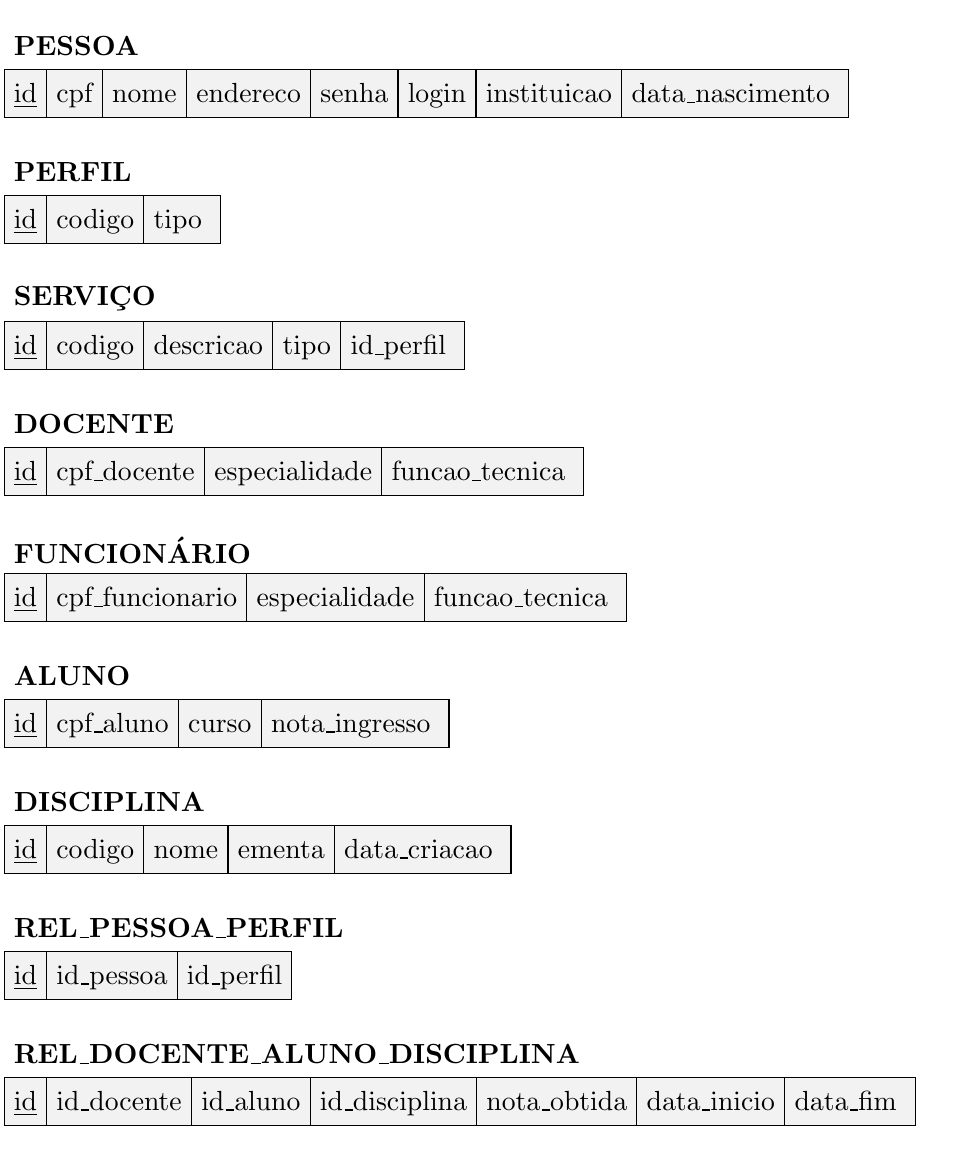
\begin{tikzpicture}[relation/.style={rectangle split, rectangle split parts=#1, rectangle split part align=base, draw, anchor=center, align=center, text height=3mm, text centered}]\hspace*{-0.3cm}

% RELATIONS

\node (pessoa-titulo) {\textbf{PESSOA}};

\node [relation=8, rectangle split horizontal, rectangle split part fill={lightgray!50}, anchor=north west, below=0.6cm of pessoa-titulo.west, anchor=west] (pessoa)
{\underline{id}%
\nodepart{two} cpf
\nodepart{three}   nome
\nodepart{four} endereco
\nodepart{five} senha
\nodepart{six} login
\nodepart{seven} instituicao
\nodepart{eight} data\_nascimento
};

\node [below=1cm of pessoa.west, anchor=west] (perfil-titulo) {\textbf{PERFIL}};

\node [relation=3, rectangle split horizontal, rectangle split part fill={lightgray!50}, below=0.6cm of perfil-titulo.west, anchor=west] (perfil)
{\underline{id}
\nodepart{two}{codigo}%
\nodepart{three} tipo
};

\node [below=1cm of perfil.west, anchor=west] (servico-titulo) {\textbf{SERVIÇO}};

\node [relation=5, rectangle split horizontal, rectangle split part fill={lightgray!50}, anchor=north west, below=0.6cm of servico-titulo.west, anchor=west] (servico)
{\underline{id}
\nodepart{two} codigo%
\nodepart{three}   descricao
\nodepart{four} tipo
\nodepart{five} id\_perfil
};

\node [below=1cm of servico.west, anchor=west] (docente-titulo) {\textbf{DOCENTE}};

\node [relation=4, rectangle split horizontal, rectangle split part fill={lightgray!50}, anchor=north west, below=0.6cm of docente-titulo.west, anchor=west] (docente)
{\underline{id}
\nodepart{two} cpf\_docente%
\nodepart{three}   especialidade
\nodepart{four} funcao\_tecnica
};

\node [below=1cm of docente.west, anchor=west] (funcionario-titulo) {\textbf{FUNCIONÁRIO}};

\node [relation=4, rectangle split horizontal, rectangle split part fill={lightgray!50}, anchor=north west, below=0.6cm of funcionario-titulo.west, anchor=west] (funcionario)
{\underline{id}
\nodepart{two} cpf\_funcionario%
\nodepart{three}   especialidade
\nodepart{four} funcao\_tecnica
};

\node [below=1cm of funcionario.west, anchor=west] (aluno-titulo) {\textbf{ALUNO}};

\node [relation=4, rectangle split horizontal, rectangle split part fill={lightgray!50}, anchor=north west, below=0.6cm of aluno-titulo.west, anchor=west] (aluno)
{\underline{id}
\nodepart{two}{cpf\_aluno}%
\nodepart{three}   curso
\nodepart{four} nota\_ingresso
};

\node [below=1cm of aluno.west, anchor=west] (disciplina-titulo) {\textbf{DISCIPLINA}};

\node [relation=5, rectangle split horizontal, rectangle split part fill={lightgray!50}, anchor=north west, below=0.6cm of disciplina-titulo.west, anchor=west] (disciplina)
{\underline{id}
\nodepart{two} codigo%
\nodepart{three}   nome
\nodepart{four} ementa
\nodepart{five} data\_criacao
};

\node [below=1cm of disciplina.west, anchor=west] (relacao-pessoa-perfil-titulo) {\textbf{REL\_PESSOA\_PERFIL}};

\node [relation=3, rectangle split horizontal, rectangle split part fill={lightgray!50}, anchor=north west, below=0.6cm of relacao-pessoa-perfil-titulo.west, anchor=west] (relacao-pessoa-perfil)
{\underline{id}
\nodepart{two} id\_pessoa%
 \nodepart{three} id\_perfil%
};

\node [below=1cm of relacao-pessoa-perfil.west, anchor=west] (relacao-docente-aluno-disciplina-titulo) {\textbf{REL\_DOCENTE\_ALUNO\_DISCIPLINA}};

\node [relation=7, rectangle split horizontal, rectangle split part fill={lightgray!50}, anchor=north west, below=0.6cm of relacao-docente-aluno-disciplina-titulo.west, anchor=west] (relacao-pessoa-perfil)
{
\underline{id}
\nodepart{two} id\_docente%
 \nodepart{three} id\_aluno
 \nodepart{four} id\_disciplina%
 \nodepart{five} 
nota\_obtida
\nodepart{six} 
 data\_inicio
\nodepart{seven} 
 data\_fim
};


\end{tikzpicture}

\end{document}
